\documentclass[10pt]{amsart}
\usepackage{geometry}                % See geometry.pdf to learn the layout options. There are lots.
\geometry{letterpaper}                   % ... or a4paper or a5paper or ... 
%\geometry{landscape}                % Activate for for rotated page geometry
%\usepackage[parfill]{parskip}    % Activate to begin paragraphs with an empty line rather than an indent
\usepackage{graphicx}
\usepackage{amssymb}
\usepackage{epstopdf}
\DeclareGraphicsRule{.tif}{png}{.png}{`convert #1 `dirname #1`/`basename #1 .tif`.png}

\title{\large{Improving the Efficiency of RRT in Heterogenous Environments with Context Sensitivity}\\~\\\small{Project Proposal}\\\small{Graduate Artificial Intelligence, Spring 2010}}
\author{Filipe Milit\~{a}o, Karl Naden, Bernardo Toninho}

\begin{document}
\maketitle

This project proposal is based off of an observation about the extension length used in the RRT \cite{Bruce02real-timerandomized} family of algorithms.  In particular, we note that for RRT to be effective, the extension length must be calibrated to the particular environment that a robot is trying to plan in.  In fig. 1, for example, the narrow passages in the wall mean that the extension length must be small.  However, this goes against one of the strengths of the RRT algorithm which is that global reasoning about the environment is not necessary.  As long as I have a map which I can use to test if a given vector is obstacle free, I don't need to discover or reason about global properties of the world.

\begin{figure}
\begin{center}
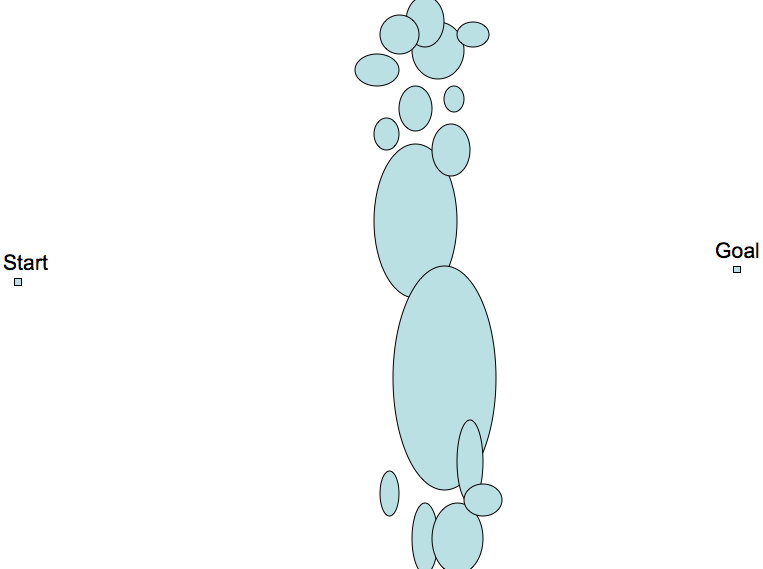
\includegraphics[width=3in]{space.png}
\end{center}
\end{figure}

One potential way to address this issue is to allow the length of the expansion distance to change over the course of the (re)planning. 
Our idea is that associating an extension factor with each point in the random tree provides information that can be used to
improve both RRT planning and re-planning. 
The basic planning algorithm would behave something like this:
\begin{enumerate}
\item Choose a random point in the world and find the nearest point in the plan tree
\item Choose an extension distance based on the extension factor of this point
\item if the expansion fails (there was an obstacle), decrease the point's extension factor and go-to (1)
\item if the expansion succeeds, increase the start point's extension factor and set the extension factor of the new node in the tree with the factor of the previous old point.
\end{enumerate}
We hypothesize that this would allow for the RRT algorithm to better handle heterogeneous spaces because it could accelerate across open spaces with larger steps, but navigate through constrained spaces as well. Furthermore, the extension factor information can be used to inform a re-planning procedure. Since the extension factor is a function of how obstructed the world
around a point is, we can use this information to approximate the set of the unobstructed regions of the world and further improve
our successive plans (i.e. if we select a point in the tree that falls into a large unobstructed region, we probably can afford larger extensions from that point).

There are three portions of this project which we think will require significant thought and programming:
\begin{enumerate}
\item {\it The basic algorithm:}  Designing and coding the basic algorithm for a single iteration will be an important piece of the project.  Determining the best way to increment and decrement the extension factor will be an interesting challenge.  Furthermore, it may well be that the simple algorithm outlined above will not work perfectly.  However, we may be able to enhance it with ideas such as associating directions with our extension factor (i.e only increase it when heading in the same or similar direction), by including the expansion multiplier in the determination of the closest point, or another scheme.
\item {\it Applying the gathered information to re-planning:} Apart from implementing the waypoints already used in ERRT, this portion of the project entails developing a way of extrapolating from the the several regions that make up the world and finding appropriate ways of using these regions as input to the extension factor changes (as summarized above). Another important part of this component is finding out how to adjust these regions, as the number of planning iterations increases and we obtain more information.

\item {\it Testing and performance metrics:} To evaluate the performance of our algorithm, we will implement a test suite (with visualization) that will allow us to measure the performance of our re-planner (in successful plans to the goal and number of steps in a plan) in several types of randomly generated worlds (worlds with uniform distributions of obstacles, non-uniform, etc.), as well as compare its performance to that of ERRT in the same
scenarios.
\end{enumerate}

We intend to each be responsible for developing one of these parts of the project. However, given that all the parts are interconnected, each of us
will naturally contribute to all components of the project.



Some other papers describing extensions to the RRT algorithm which may be helpful include \cite{Lavalle98rapidly-exploringrandom},\cite{Lindemann04incrementallyreducing},\cite{Jaillet05adaptivetuning}, and \cite{moplan2009}.
\bibliography{AIbib}{}
\bibliographystyle{plain}
\end{document}